
%(BEGIN_QUESTION)
% Copyright 2010, Tony R. Kuphaldt, released under the Creative Commons Attribution License (v 1.0)
% This means you may do almost anything with this work of mine, so long as you give me proper credit

Skisser {\it pumpekurven} for en fortrengningspumpe som drives med konstant hastighet av en elektrisk motor:

$$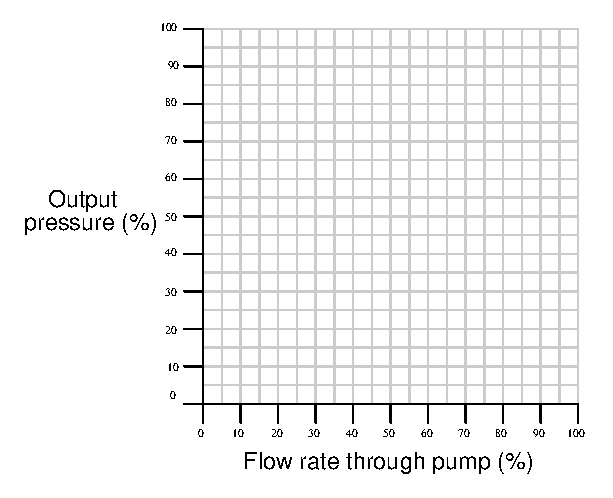
\includegraphics[width=15.5cm]{i00743x01.eps}$$

\vskip 20pt \vbox{\hrule \hbox{\strut \vrule{} {\bf Forslag til sokratisk diskusjon} \vrule} \hrule}

\begin{itemize}
\item{} Hva vil endre seg i pumpekurvegrafen dersom hastigheten på drivmotoren endres?
\end{itemize}

\underbar{file i00743}
%(END_QUESTION)





%(BEGIN_ANSWER)

Den ideelle pumpekurven for en fortrengningspumpe er en vertikal linje, men på grunn av intern lekkasje ser den reelle pumpekurven mer slik ut:

$$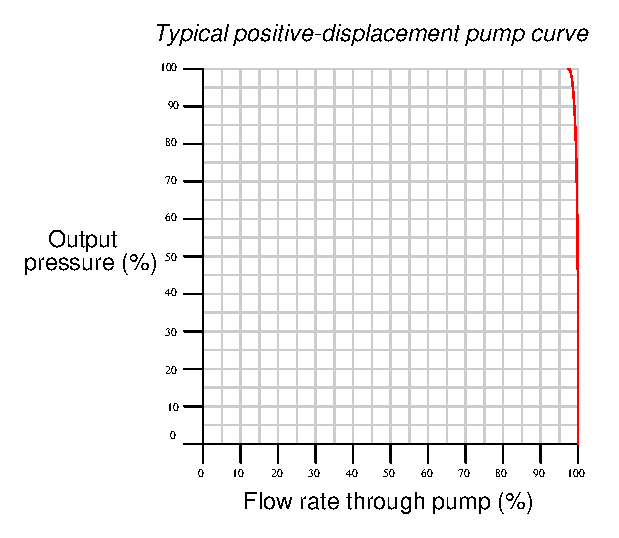
\includegraphics[width=15.5cm]{i00743x02.eps}$$

%(END_ANSWER)





%(BEGIN_NOTES)


%INDEX% Sluttkontrollelementer, pumpe: trykk/flow-kurve

%(END_NOTES)

